\begin{figure}
\centering
    % \begin{minipage}{0.48\linewidth}
    \begin{subfigure}{0.32\linewidth}
        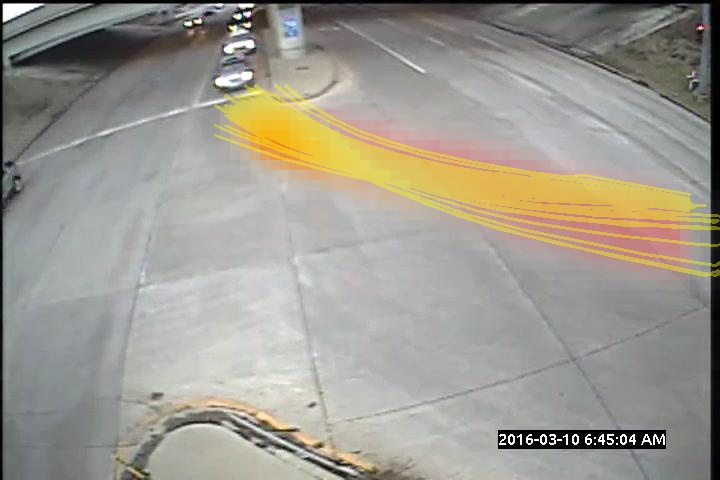
\includegraphics[width=\linewidth]{./img/scene_learning/ridges-1.jpg}
        \subcaption{}
        \label{subfig:scene-ridges}
    \end{subfigure}
    \begin{subfigure}{0.32\linewidth}
        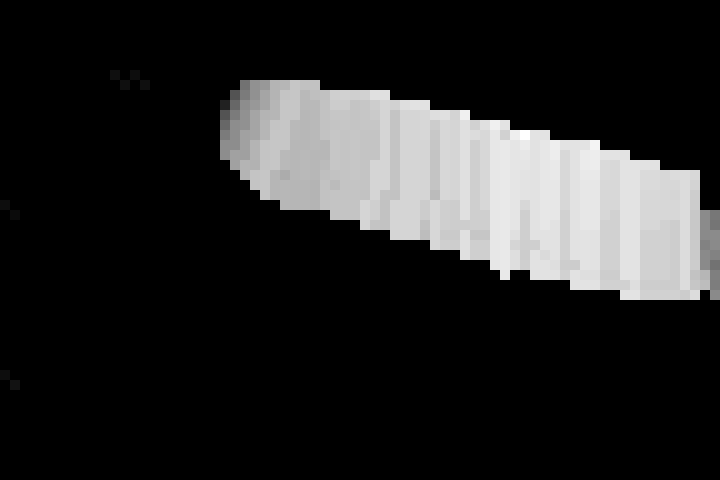
\includegraphics[width=\linewidth]{img/scene_learning/perp_width-1.png}
        \subcaption{}
        \label{subfig:scene-perp-width}
    \end{subfigure}
    \begin{subfigure}{0.32\linewidth}
        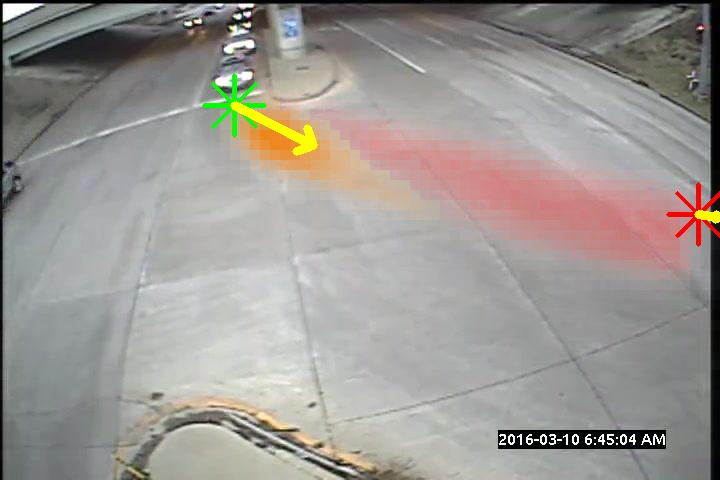
\includegraphics[width=\linewidth]{./img/scene_learning/res/middle/middle-1.jpg}
        \subcaption{}
        \label{subfig:scene-entry-exit}
    \end{subfigure}%
    \caption{(\subref{subfig:scene-ridges}): multiple ridges learned from local maximal grid. (\subref{subfig:scene-perp-width}): perpendicular width, where lighter intensity indicates a larger width. (\subref{subfig:scene-entry-exit}): extracted entry/exit hotspots indicates by the green and red star. And the yellow arrow shows their direction.}
    \label{fig:scene-ridge-res}
    % \end{minipage}
\end{figure}